\documentclass[11pt, letterpaper, onecolumn, oneside, final]{article}

\usepackage{lab}
\usepackage{soul}

\newfontfamily{\consolas}{Consolas}[Extension = .ttf]

\DocumentTitle {Project 2}
\DocumentSubtitle {Text Analysis}
% End of preamble

%%%%%%%%%%%%%%%%%%%%%%%%%%%%%%%%%%%%%%%%%%%%%%%%%%%%%%%%%%%%%%%%%%%%%%%

\begin{document}
    \maketitle

    %\duedate{Weekday assigned: 0-6}{Week assigned: 0}{Weekday due:0-6}{Week due: 1}{Time due: 10:00 p.m.}
    \duedate{4}{0}{0}{3}{10:00 p.m.}

    \section{Collaboration.} Reminder of the collaboration policy: you may discuss the ideas of the project, but cannot share code or look at another student’s code. If you discuss, cite. More details are in the course syllabus. 

    \section{Introduction.} In this project, you will be exploring the {\consolas matplotlib} and {\consolas nltk} modules in order to create an interactive text analysis toolkit. 
     
     
     
     %Begin by downloading the necessary skeleton code ({\consolas language.py}) found on the resources page on the class Piazza page. You can find them on the Resources page under Projects. Place them in a Project2 folder in the Projects folder in your CS101 directory.
    \section{What to do.}  You can create and then open {\consolas language.py} in Thonny and begin the project. Be sure to save regularly, in case of any mishaps. Make sure to pay attention to the comments already in the file. Make sure you import both the {\consolas nltk} and {\consolas matplotlib} modules, as you did at the beginning of Lab 2A.\\
    \\
% Should we give them code for the menu or should they just have to write that code? %
  Your task is to implement a series of at least two tools that can be used to manipulate and analyze any given text, using the standard input stream. You will need to use a loop to display an interactive menu, from which any one of your functions can be selected. This interactive menu will display several numbered tools from which the user can choose. The user will then be prompted to enter a number or a string, and the corresponding tool will be run. It should look something like this:
  \begin{center}
  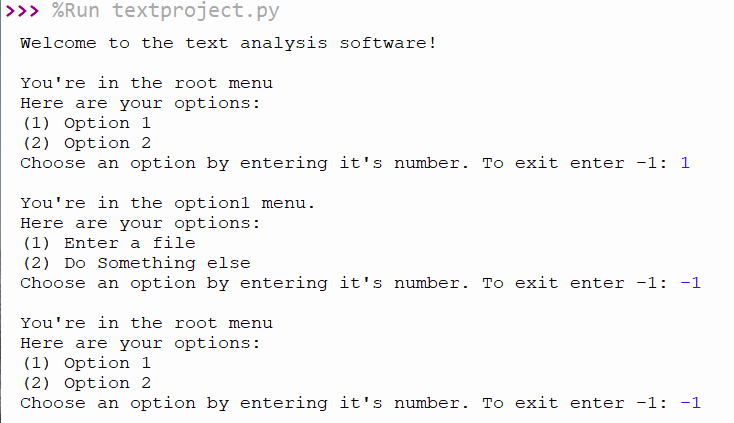
\includegraphics[scale=.5]{textmenu2}
  \end{center}
  If you need further clarification on how to operate this menu or how to handle the standard input stream, TA hours are a great resource.
  \newpage
  You can design any tool that you would like that uses the {\consolas matplotlib} and {\consolas nltk} modules. If you are struggling to come up with ideas, some tools you might implement include:
  \begin{itemize}
      \item \textbf{A MadLibs Generator}: Create a randomly generated MadLibs puzzle by removing a particular part of speech.
%        \begin{itemize}
            \item \textbf{A MadLibs Solver}: Fill in the puzzle randomly by adding the correct parts of speech from other parts of the text.
%        \end{itemize}
      \item \textbf{A Character Tracker}: Given a character, track their occurrences throughout the text and use plots to display the data. 
%      \begin{itemize}
          \item \textbf{A Relationship Tracker}: Have the user input multiple characters and track their relationship, interactions, and frequencies throughout the text.
%      \end{itemize}
      \item \textbf{Part of Speech Analyzer}: Track the frequencies of the various parts of speech throughout a given piece of text.
%      \begin{itemize}
          \item \textbf{Part of Speech Frequency}: Create a plot of most frequent words of a given type of speech in the entire text.
%      \end{itemize}
      \item \textbf{Another Option}: You can also combine parts of multiple tools to do other interesting things. For example, you could get a list of all of a character's occurrences in a text then use parts of speech analysis to check if the words around each occurrence are adjectives, and keep track of the adjectives most used to describe that character. 
  \end{itemize}
  \\
  You may use anything from labs and lecture to create this toolkit, but be sure to cite when necessary. If you would like further documentation on {\consolas matplotlib}, visit \textcolor{blue}{\underline{https://matplotlib.org/index.html}}. If you would like further documentation on {\consolas nltk}, visit \textcolor{blue}{\underline{http://www.nltk.org}} or \textcolor{blue}{\underline{http://www.nltk.org/book/}}. If you need further clarification on the parts of speech as generated by the {\consolas nltk} module, visit \textcolor{blue}{\underline{https://sites.google.com/site/partofspeechhelp/#TOC-IN}}. As a reminder, here is what a citation should look like: \\ 
    \\
    \indent{\consolas \# CITE: https://docs.python.org/3/library/turtle.html}\\
    \indent{\consolas \# DETAILS: Looked up how to change the background color.}\\ 
    \\
    Your final product should demonstrate your understanding of while loops and for loops, Boolean logic, string methods and slicing, standard input/output streams, and the {\consolas matplotlib} and {\consolas nltk} modules.
    Submissions that reflect a deeper understanding or more interesting use of these techniques will be graded more favorably. Some options to display a more advanced grasp on the topics include:
\begin{itemize}
    \item Use of {\consolas matplotlib} or {\consolas nltk} functions not taught in lab
    \item Creative text analysis techniques not described above
    \item Applications of Lab 2B or Lab 2C material.
\end{itemize}
    Refer to the grading rubric for more grading information.
    
\section{How to submit.}

    Submit your project to Gradescope using the standard course submission procedures. 
    \section{Grading Rubric:} 
    \begin{enumerate}
        \item \textbf{Creativity}: Don't just stick to the project ideas given above, but rather use those as a starting point of what you could do. Aim to expand on those ideas and/or integrate them into an original idea of your own.
        \item \textbf{Effective use of {\consolas nltk} and {\consolas matplotlib} methods}: Display that you not only know how to use these two modules but you know how to use them together in order to achieve a goal. 
        \item \textbf{Use of Boolean statements}: Use effective and efficient Boolean statements to guide the control flow of your program. We want to see that your code can account for changes in input.
        \item \textbf{Advanced use of loops}: Demonstrates a more advanced understanding of looping structures than required in previous projects, such as more intricate for loops and while loops.
        \item \textbf{Data analysis}: Display that you are able to take a set of raw data and extract meaningful information from it to accomplish a given task.
        \item \textbf{Function definition \& use}: Demonstrates an understanding of function definition and implementation as a means to streamline code. Must be able to create and use their own functions that require one or more parameters.
    \end{enumerate}
    \section{Important Notes:} 
    \begin{enumerate}
        \item A satisfactory project will incorporate both the {\consolas nltk} and the {\consolas matplotlib} modules completely and consistently. The quality of your tools is worth as much as the quantity; we would rather see two high-quality tools than four mediocre ones. The effective use of computer science concepts is worth more than the overall aesthetic of the final output. We want to see you experiment and be creative with both your final project \emph{and} the code that you use to produce it. The amount of effort put into this project will be clear, and the project will be graded accordingly.
        \item You must be able to explain your code in a reasonable amount of detail to the grader that you will be meeting with. This will demonstrate to them that you understand the code that you have written. If you are unable to talk through your code, it is probably a sign that you need to visit TA hours or stop into your Professor's office hours for clarification. 
    \end{enumerate}

    
\end{document}